%\begin{center}
%     \Large{\textbf{AND Cheat Sheet}} \\
%\end{center}

%\section{Vocabulary}
%\textsc{Hyperbolic eq.points} $\Re\{\lambda\} \neq 0$ \\
%\textsc{Nonhyperbolic problems} Equilibria with EV on the imaginary axis.\\

\section{Basics on cont.-time dynamical systems}
\begin{align*}
\dot{x} = f(t,x,p), \quad x(t_0) = x_0 \Leftrightarrow \dx = f(x,p), \quad x(0)=x_0
\end{align*}
\subsection{Flow of a system}
Solution is the flow $\phi_t(x_0)$
\begin{align*}
x(t;x_0,p)=\phi_t(x_0,p)
\end{align*}
\textsc{Flow axioms}\\
\begin{align*}
\phi_0(x_0,p)&=x_0\\
\phi_{t_1}[\phi_{t_2}(x_0,p),p] &= \phi_{t_1+t_2}(x_0,p)
\end{align*}
\subsection{Existence and uniqueness}
\textsc{Existence and uniqueness of local (in time) solutions}\\
\emph{If $f(x)$ is smooth enough, then solutions exist and are unique. No guarantee that they exist forever - only guarantees to exist in a very short time interval around $t_0$.}\\
If $f$ is Lipschitz in $x$ and piecewise continuous in $t$ then the IVP has a unique solution $x(t)=\phi(t;t_0)x_0$ over a finite time interval $t\in[t_0-\tau,t_0+\tau]$.\\
Allows for finite-escape times/blow-up (reach infinity in finite time).

\subsection{Stability}
Def.: An equilibrium point is a state $x^*$ s.t. $f(x^*)=0$\\
Def.: An eq.point $x^*$ is stable if for any $\epsilon>0$ there exists a constant $\delta > 0$ such that \begin{align*}
\forall x_0: \Vert x_0 - x^* \Vert \leq \delta \Rightarrow \Vert x(t)-x^* \Vert \leq \epsilon \quad \forall t \geq 0
\end{align*}

\textsc{Attractor}\\
$x^*$ is attractive if $\lim_{t\rightarrow \infty} \Vert x(t)-x^* \Vert = 0 \quad \forall x_0 \in \mathcal{S}$ with $\mathcal{S}$ being the domain of attraction.\\
Eq points may be attractive without being stable (ex. Vinograd's system).

\textsc{Asymptotic stability}\\
An eq.point $x^*$ is asymptotically stable if it is stable and attractive.

\textsc{Exponential stability}\\
An eq.point $x^*$ is exponentially stable in $\mathcal{S}$ if it is stable and there are constants $a, \lambda > 0$ such that $\forall x_0 \in \mathcal{S}: \Vert x(t)-x^*\Vert \leq a\Vert x_0 - x^* \Vert e^{-\lambda t}$

\section{Linear systems}
\subsection{LTI Systems}
\[ \dot{x} = f(x,u) \rightarrow \dot{x} = Ax \]
mit $A \in \mathbb{R}^{n \times n}$ linear map/transformation

Theorem:
The origin of the linear system is stable if all EV $\lambda_i$ have non positive real part. If all EV have negative Real part, the origin is exponentially stable.

\[ \lambda^2+tr(A)\lambda+det(A) = 0 \]
%\[ tr(A) = a_{11} + a_{22} \]
%\[ det(A) = a_{11}a_{22} - a_{12}a_{21} \]

\[ \lambda_{1,2} = \frac{1}{2} \left( tr(A) \pm \sqrt{tr(A)^2-4det(A)}\right) \]

daraus folgt
$tr(A) < 0 \rightarrow$ stable\\
$tr(A) > 0 \rightarrow$ unstable\\
$tr(A)^2 \geq 4det(A)$ node\\
$tr(A)^2 < 4det(A)$ spiral\\
$det(A) < 0 \rightarrow$ saddle

Spezialfall:
$tr(A)^2 = 4det(A)$ $\rightarrow$ stable if $tr(A) < 0$\\


%\begin{pspicture}(6,5)
%    \psline{->}(0,2)(5,2) \rput*(5.5,2){det}
%    \psline{->}(2,0)(2,4) \rput*(2,4.2){tr}
%    \rput(3.2,4){unstable node}
%    \rput(3.5,2.5){unstable spiral}
%    \rput(3.5,1.5){stable spiral}
%    \rput(3,0.5){stable node}
%    \rput(0.5,2.5){saddles}
%    \rput(0.5,1.5){saddles}
%    \pscurve(4.5,3.5)(2,2)(4.5,0.5)
%\end{pspicture}

\subsection{LTV Systems and Floquet theory}
Periodic matrix $A(t)$, such that $A(t+T)=A(t), \; \forall t \geq 0$. The fundamental matrix $P(t)$ satisfies $P(t+T)=P(t)M, \quad M=P^{-1}(t_0)P(T)$, with $M=e^{TB}$ for some matrix $B$. The EVs of $M$ are called Floquet multipliers and the EVs of $B$ are called Floquet exponents.\\
\textbf{Calculate Floquet MPs}\\
Solve $\dot{P}(t)=A(t)P(t), \; P(t_0)\neq 0$ with initial condition $P(0)=I$\\
Floquet MPs are the EVs of $M=P(T)$ and Floquet Exps are the EVs of $B=\frac{1}{T}\ln M$

\section{Nonlinear Flows}
\subsection{Local Theory}
\textsc{Hartman-Grobman}\\
The behavior of a nonlinear systems in a vicinity of hyperbolic eq. points is the same as in the linearized system around that point.
\emph{Hyperbolic}: $EV of J(x^*,p) \neq 0$
\vspace{0.2cm}

\textsc{Center manifold theorem}\\

\begin{enumerate}
\item Write the system in diagonal form:
\begin{align*}
\dot{x}=Cx+F(x,y)\\
\dot{y}=Py+G(x,y)
\end{align*}
\item Determine $h(x)=ax^2+bx^3+...$
\item Has to satisfy
\begin{align*}
Dh(x)[Cx+F(x,h(x))]=Ph(x)+G(x,h(x))
\end{align*}
\item Collect terms $\mathcal{O}^i$ and determine constants $a,b,...$ to set them to zero
\item Insert constants into $h(x)$
\item Calculate $\dot{x}=Cx+F(x,h(x))$
\end{enumerate}


\subsection{Non-local phenomena}
\subsubsection{Index theory}
\emph{Linearization gives only microscopic view around a fixed point - it fails especially at higher order terms. Use index theory for global information about phase portrait.}\\
Index $I_C$ of a closed curve $C$ describes the number of counterclockwise revolutions made by the vector field as $x$ moves once counterclockwise around $C$.\\
\textbf{Properties:}\\
$I_C=0$ if $C$ doesn't enclose any EQPs\\
Time reversal does not change the index\\
If $C$ is a trajectory (e.g. closed orbit), then $I_C=+1$.\vspace{0.1cm}
\textbf{Properties of indexes of points:}\\
$I_C=\sum_{i=1}^k I[x_{i*}]$\\
stable, unstable node $I_C = -1$\\
s/u spiral $I_C = 1$\\
s/u limit cycle $I_C = 1 \rightarrow$ wegen EQP im Kern
\subsubsection{Limit Cycles}
Nonlinear, non-local phenomenon. Limit cycle is isolated. A linear center is surrounded by a continuum family of periodic orbits. A limit cycle necessarily encloses at least one EQP.

\textsc{Lineard}\\
$\ddot{x}+f(x) \dot{x} + g(x)=0$ has a unique stable LC surrounding the origin if:\\
\textbf{(1)} $f(x)$ and $g(x)$ are cont.diff. $\forall x$, \textbf{(2)} $g(x)$ odd, \textbf{(3)} $g(x)>0$ for $x>0$, \textbf{(4)} $f(x)$ even and \textbf{(5)} $F(x)=\int_0^x f(u)du$ has exactly one zero at $x=a$ is $<0$ for $0<x<a$ and $>0$ and nondecreasing for $x>a$ and $F(x)\rightarrow\infty$ as $x\rightarrow \infty$.\vspace{0.2cm}

\textsc{Poincare Bendixson}\\
Let $x(t)$ be a trajectory of a dynamic system, which evolves within a compact set $M$ (trapping region). Then $x(t)$ converges either to an equilibrium point, or to a closed orbit.\vspace{0.2cm}

\textsc{Bendixon-Dulac's criterion}\\
Let $D$ be a subset. If there exists a $C^1$ function $\phi(x)$ such that $\nabla(\phi\dot{x})$ does not change sign over $D$, then there are no closed traj. in $D$. Choose $\phi$ as e.g. $1, 1/x^ay^b,\, e^{ax},\,e^{ay}$.

\textsc{Lyapunov functions}\\
If a Lyapunov function $V(x)$ (cont.diff, real-valued) exists it excludes the existence of limit cycles. Suppose $x^*$ and the properties \textbf{(1)} $V(x)>0$ for all $x\neq x^*$ and $V(x^*)=0$ (pos.def.) and \textbf{(2)} $\dot{V}<0$ for all $x\neq x^*$ 

\section{Bifurcations of vector fields}
\subsection{Bifurcations of SSs}
\textsc{Transcritical bifurcation}\\
\emph{Standard mechanism for change of stability for a fixed point which exists for all values of the parameter}.\\
Ex.: $\dot{x}=rx-x^2$.\\
Fixed point at $x^*=0 \quad \forall r$. For $r<0$ unstable fixed point at $x^*=r$ and a stable at $x^*=0$. For $r=0^-$ the fixed points unify. For $r>0$ the origin is unstable and $x^*=r$ becomes stable - \textbf{exchange of stabilities}
\begin{center}
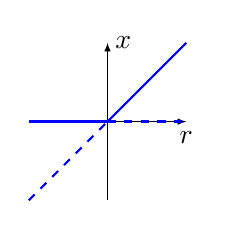
\begin{tikzpicture}
\draw [ultra thin,latex-](0,1.5) -- (0,-0.5);
\draw [ultra thin,-latex](-1,0.5) -- (1,0.5);
\draw [color=blue,thick](-1,0.5) -- (0,0.5);
\draw [color=blue,dashed,thick](0,0.5) -- (1,0.5);
\draw [color=blue,thick](0,0.5) -- (1,1.5);
\draw [color=blue,dashed,thick](-1,-0.5) -- (0,0.5);
\node at (1,0.3) {$r$};
\node at (0.2,1.5) {$x$};
\end{tikzpicture}
\end{center}
\vspace{0.2cm}


\textsc{Saddle node bifurcation}\\
\emph{Fixed points are created and destroyed. As a parameter is varied, two fixed points move toward each other, collide and mutually annihilate}.\\
Ex: $\dot{x}=r+x^2$.\\ $r<0$: 2 FP (1 stable, 1 unstable),\\ $r=0^-$: half-stable FP, \\ $r>0$: no FP.\\ In this example the bifurcation occurred at $r=0$.
\begin{center}
\begin{tikzpicture}
\draw [ultra thin,latex-](0,1.5) -- (0,-0.5);
\draw [ultra thin,-latex](-1,0.5) -- (1,0.5);
\draw [color=blue,thick](-1,-0.25) .. controls (-0.5,-0.1) and (0,0) .. (0,0.5);
\draw [color=blue,dashed](-1,1.25) .. controls (-0.5,1.1) and (0,1) .. (0,0.5);
\node at (1,0.3) {$r$};
\node at (0.2,1.5) {$x$};
\end{tikzpicture}
\end{center}
\vspace{0.2cm}

\subsubsection{Pitchfork bifurcation}
\emph{Common in physical systems that have (left/right) symmetry.}
\textsc{Supercritical pitchfork bifurcation}\\
Ex: $\dot{x}=rx-x^3$. If $r<0$ the origin is the only fixed point and stable. $r=0$ the origin is still stable, but weakly, since the linearization vanishes (solutions no longer decay exponentially fast - \emph{critical slowing down}).  For $r>0$ the origin becomes unstable and two new stable fixed points appear at $x^*=\pm \sqrt{r}$.
\begin{center}
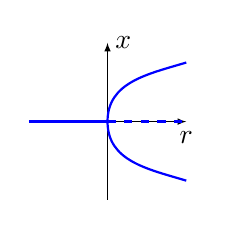
\begin{tikzpicture}
\draw [ultra thin,latex-](0,1.5) -- (0,-0.5);
\draw [ultra thin,-latex](-1,0.5) -- (1,0.5);
\draw [color=blue,thick](-1,0.5) -- (0,0.5);
\draw [color=blue,dashed,thick](0,0.5) -- (1,0.5);
\draw [color=blue,thick](1,-0.25) .. controls (0.5,-0.1) and (0,0) .. (0,0.5);
\draw [color=blue,thick](1,1.25) .. controls (0.5,1.1) and (0,1) .. (0,0.5);
\node at (1,0.3) {$r$};
\node at (0.2,1.5) {$x$};
\end{tikzpicture}
\end{center}
\vspace{0.2cm}

\textsc{Subcritical pitchfork bifurcation}\\
Ex: $\dot{x}=rx+x^3$. Only for $r<0$ two unstable fixed points $x^*=\pm \sqrt{-r}$ and stable origin. For $r>0$ origin is unstable (finite escape)
\begin{center}
\begin{tikzpicture}
\draw [ultra thin,latex-](0,1.5) -- (0,-0.5);
\draw [ultra thin,-latex](-1,0.5) -- (1,0.5);
\draw [color=blue, thick](-1,0.5) -- (0,0.5);
\draw [color=blue,dashed](0,0.5) -- (1,0.5);
\draw [color=blue,dashed](-1,-0.25) .. controls (-0.5,-0.1) and (0,0) .. (0,0.5);
\draw [color=blue,dashed](-1,1.25) .. controls (-0.5,1.1) and (0,1) .. (0,0.5);
\node at (1,0.3) {$r$};
\node at (0.2,1.5) {$x$};
\end{tikzpicture}
\end{center}

%\subsubsection{Bifurcations of SSs in dim $n>1$}
%\begin{align*}
%\text{transcritical bif: }& \dot{x}_1=rx_1-x_1^2 \quad &\dot{x}_2 = \pm x_2 \\
%\text{saddle-node bif: }& \dot{x}_1 = r-x_1^2, \quad &\dot{x}_2 = \pm x_2\\
%\text{pitchfork bif: }& \dot{x}_1=rx_1-x_1^3, \quad &\dot{x}_2 = \pm x_2
%\end{align*}

\subsection{Bifurcations of trajectories}
\textsc{Flows on the circle}\\
Vector field on the circle $\dot{\Theta}=f(\Theta)$, with $\Theta$ being a point on the circle. Particle can return to starting place - most basic model of oscillating systems.\\

\textsc{Non-uniform oscillator}\\
$\dot{\Theta} = \omega - p\sin \Theta$ with mean $\omega$ and amplitude $a$.\\
\textbf{Uniform oscillator $p=0$}: $\dot{\Theta} = \omega$ and $\omega=\text{const.}$ with solution $\Theta(t)=\omega t + \Theta_0$. \emph{Phase $\Theta$ changes uniformly}.\\
%\begin{center}
%\begin{tikzpicture}
%\draw (-1,1.5) -- (-1,-0.5);
%\draw (-1,0.5) -- (3.5,0.5);
%\node at (3.5,0.3) {$t$};
%\node at (-0.8,1.5) {$\Theta$};
%\draw (-1,0) -- (0.5,1.5) -- (0.5,-0.5) -- (2.5,1.5) -- (2.5,-0.5) -- (3.5,0.5);
%\end{tikzpicture}
%\end{center}

For $0<p<\omega$ there is a non uniform oscillation, because the velocity depends on the angle. For $p=\omega$ a SS appears at $\Theta=\sfrac{\pi}{2}$ attracting the flow from one side and repelling the other side. For $p>\omega$ there are two SSs (1 repulsor, 1 attractor).\\
For $p\lesssim\omega$ there exists a saddle-note ghost. Time to pass through the bottleneck via local rescaling around the bottleneck: $\dot{x}=r+x^2$ where $0<r = \frac{2(\omega-p)}{p}\ll 1$ is proportional to the distance of the bif. $T\approx
\int_{-\infty}^{\infty} \frac{dx}{r+x^2} = \frac{\pi}{\sqrt{r}}$

\begin{center}
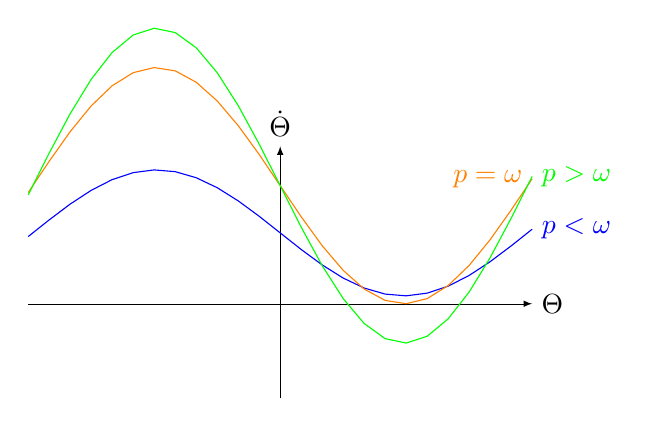
\begin{tikzpicture}[domain=-3.2:3.2]
\draw[ultra thin,-latex] (-3.2,0) -- (3.2,0) node[right] {$\Theta$};
\draw[ultra thin,-latex] (0,-1.2) -- (0,2) node[above] {$\dot{\Theta}$};
\draw[color=blue] plot (\x,{0.9-0.8*sin(\x r)}) node[right] {$p<\omega$};
\draw[color=orange] plot (\x,{1.5-1.5*sin(\x r)}) node[left] {$p=\omega$};
\draw[color=green] plot (\x,{1.5-2*sin(\x r)}) node[right] {$p>\omega$};
\end{tikzpicture}   
\end{center}

\subsubsection{Andronov-Hopf bifurcation (2D)}
\emph{No SSs appear/disappear. Rather the behaviour changes qualitatively for small variations, e.g. decaying oscillation vs. increasing oscillation with limiting amplitude after the bifurcation.}\\
Can occur in phase spaces of any dimension $n\geq 2$.

\textsc{Supercritical Hopf bifurcation}\\
Decay rate dependent on control parameter $p$. Decay becomes slower and slower and finally changes to a growth at a critical $p_c$ (equilibrium becomes unstable). In many cases there results a limit cycle about the former SS. \textbf{In phase plane:} Stable spiral becomes unstable spiral surrounded by a small nearly elliptical limit cycle.
Example:
\begin{align*}
\dot{r}=pr-r^3\\
\dot{\Theta}=\omega+br^2
\end{align*}
with control parameter $p$, $\omega$ frequency and $b$ as dependence of frequency on amplitude. Stable spiral for $p<0$ in origin $r=0$ and sense of rotation depends on $\omega$. For $p=0$ the origin is very weakly stable. For $p>0$ there is an unstable spiral at the origin and a stable limit cycle at $r=\sqrt{p}$.\\
EV analysis via cartesian coordinates $x_1=r\cos \Theta$, $\;x_2=r\sin \Theta$ yields $\dot{x}_1 = px_1-\omega x_2$, $\quad\dot{x}_2 = \omega x_1+p x_2$ with the Jacobian $J=\begin{bmatrix}
p & -\omega \\ \omega & p
\end{bmatrix}$ and $\lambda_{1,2} = p \pm i\omega$. EVs cross the imaginary axis from left to right as $p$ increases from - to +. \\
\textbf{Rules of thumb:} Size of limit cycle grows from 0 proportionally to $\sqrt{p-p_c}$. Frequency of limit cycle $\omega \approx \Im \{\lambda\}$ evaluated at $p=p_c$.
\begin{center}
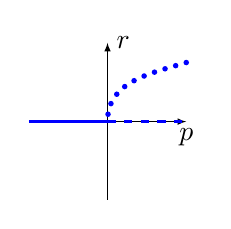
\begin{tikzpicture}
\draw [ultra thin,latex-](0,1.5) -- (0,-0.5);
\draw [ultra thin,-latex](-1,0.5) -- (1,0.5);
\draw [color=blue,thick](-1,0.5) -- (0,0.5);
\draw [color=blue,thick,dashed](0,0.5) -- (1,0.5);
\draw [color=blue,line width=2, line cap=round, dash pattern=on 0pt off 2\pgflinewidth] (1,1.25) .. controls (0.5,1.1) and (0,1) .. (0,0.5);
\node at (1,0.3) {$p$};
\node at (0.2,1.5) {$r$};
\end{tikzpicture}
\end{center}
\vspace{0.2cm}

\textsc{Subcritical Hopf bifurcation (More Dangerous)}\\
\emph{Stable origin surrounded by unstable limit cycle which collapses at $p=0$ leading to a repulsive spiral with no saving limit cycle around.}\\
Example:
\begin{align*}
\dot{r}=pr+r^3\\
\dot{\Theta}=\omega+br^2
\end{align*}
Cubic term is destabilizing yielding a stable origin and a unstable unstable limit cycle at $r=-\sqrt{-p}$ only existing for $p<0$. Unstable for $p\geq 0$ (weakly at $p=0$).
\begin{center}
\begin{tikzpicture}
\draw [ultra thin,latex-](0,1.5) -- (0,-0.5);
\draw [ultra thin,-latex](-1,0.5) -- (1,0.5);
\draw [color=blue,thick](-1,0.5) -- (0,0.5);
\draw [color=blue,thick,dashed](0,0.5) -- (1,0.5);
\draw [color=blue,line width=2.1, line cap=round, dash pattern=on 0pt off 2\pgflinewidth](-1,1.25) .. controls (-0.5,1.1) and (0,1) .. (0,0.5);
\draw [color=white,line width=2.1, line cap=round, dash pattern=on 0pt off 2\pgflinewidth](-1,1.25) .. controls (-0.5,1.1) and (0,1) .. (0,0.5);
\node at (1,0.3) {$p$};
\node at (0.2,1.5) {$r$};
\end{tikzpicture}
\end{center}
\vspace{0.2cm}

\textsc{Degenerate Hopf bifurcation}\\
\emph{Conj. complex EV pass through the imaginary axis, but do not isolated periodic orbits (limit cycle).}\\
Linear system example:
\begin{align*}
\dot{x}_1=px_1-x_2\\
\dot{x}_2=x_1+px_2\\
\end{align*}
Nonlinear example, inverted pendulum with Coulomb friction $\ddot{\Theta}+\rho \dot{\Theta} + k\sin \Theta = 0$. For $p<0$ stable spiral, a center (\emph{no limit cycles}) for $p=0$ (band of closed orbits) and unstable spiral for $p>0$.

\subsubsection{Bifurcation of limit cycles}
\textsc{Infinite period bifurcation}\\
Example:
\begin{align*}
\dot{r}=r-r^2\\
\dot{\Theta}=p-\Theta^2
\end{align*}
Two radial equilibrium solutions $r=0$ and $r=1$ (attractive). For $p<0$ no angular eq.point exists so that the limit cycle $r=1$ is a unique attractor, attracting trajectories from unstable origin. For $p=0$ a SS at $(r,\Theta)=(1,0)$ appears similar to a saddle point with radial attraction ($x_1$-direction) and angular saddle behaviour - the time through the bottleneck of $p<0$ becomes infinite for $p=0$. For $p>0$ there are two SSs at $(1,\sqrt{p})$ (attractor) and $(1,-\sqrt{p})$ (repulsor) - looks like pacman.
\begin{center}
\begin{tikzpicture}
\draw [ultra thin,latex-](0,1.5) -- (0,-0.5);
\draw [ultra thin,-latex](-1,0.5) -- (1,0.5);
\draw [color=blue,thick,dashed](-1,0.5) -- (0,0.5);
\draw [color=blue,thick,dashed](0,0.5) -- (1,0.5);
\draw [color=blue,line width=2.1, line cap=round, dash pattern=on 0pt off 2\pgflinewidth](-1,1) -- (0,1);
\draw [color=white,line width=2.1, line cap=round, dash pattern=on 0pt off 2\pgflinewidth](-1,1) -- (0,1);
\draw [color=blue,thick](0,1) -- (1,1);
\node at (1,0.3) {$p$};
\node at (0.2,1.5) {$r$};
\end{tikzpicture}
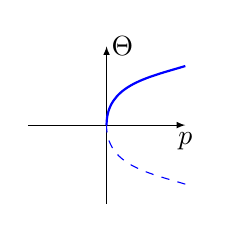
\begin{tikzpicture}
\draw [ultra thin,latex-](0,1.5) -- (0,-0.5);
\draw [ultra thin,-latex](-1,0.5) -- (1,0.5);
\draw [color=blue, dashed](1,-0.25) .. controls (0.5,-0.1) and (0,0) .. (0,0.5);
\draw [color=blue, thick](1,1.25) .. controls (0.5,1.1) and (0,1) .. (0,0.5);
\node at (1,0.3) {$p$};
\node at (0.2,1.5) {$\Theta$};
\end{tikzpicture}
\end{center}

\textsc{Saddle-node bifurcation of cycles}\\
\emph{A bifurcation in which two limit cycles unite and annihilate}.\\
Example
\begin{align*}
\dot{r}&=pr+r^3-r^5 \\
\dot{\Theta}&=\omega+br^2
\end{align*}
Radial dynamics can be seen as a 1D system with saddle-node bifurcation of SS at $p_c=-\sfrac{1}{4}$. In the 2D system they correspond to limit cycles. At $p_c$ a half-stable cycle is born. For $0>p>p_c$ it splits into a pair of limit cycles, the inner unstable and the outer stable. The other way around two limit cycles collide and disappear as $p$ decreases through $p_c$. The origin remains a stable spiral throughout.
\begin{center}
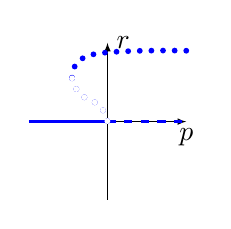
\begin{tikzpicture}
\draw [ultra thin,latex-](0,1.5) -- (0,-0.5);
\draw [ultra thin,-latex](-1,0.5) -- (1,0.5);
\draw [color=blue,thick](-1,0.5) -- (0,0.5);
\draw [color=blue,thick,dashed](0,0.5) node (v1) {} -- (1,0.5);
\node at (1,0.3) {$p$};
\node at (0.2,1.5) {$r$};
\draw [color=blue,line width=2.1, line cap=round, dash pattern=on 0pt off 2\pgflinewidth] plot[smooth, tension=.7] coordinates {(1,1.4) (-0.2,1.35) (-0.45,1.05)};
\draw [color=blue,line width=2.1, line cap=round, dash pattern=on 0pt off 2\pgflinewidth] plot[smooth, tension=.7] coordinates {(-0.45,1.05) (-0.35,0.85) (-0.1,0.7) (v1)};
\draw [color=white,line width=2.1, line cap=round, dash pattern=on 0pt off 2\pgflinewidth] plot[smooth, tension=.7] coordinates {(-0.45,1.05) (-0.35,0.85) (-0.1,0.7) (v1)};
\end{tikzpicture}
\end{center}

\vspace{0.2cm}

\textsc{Homoclinic bifurcation}\\
\emph{Part of a LC moves closer to a saddle point. At the bif the LC touches the saddle and becomes a homoclinic orbit - another kind of infinite-period bif}.\\
Example:
\begin{align*}
\dot{x}_1&=x_2\\
\dot{x}_2&=x_1 + px_2 - x_1^2 + x_1x_2
\end{align*}
$p_c=-0.86$. For $p < -1$ there is a stable spiral and a saddle node. For $p=-1$ a Hopf bifurcation. For $-1<p<p_c$ a stable LC passes close to a saddle at the origin. As $p=p_c$ the LC hits the saddle, creating a homoclinic orbit (connecting the saddle with itself). For $p>p_c$ the saddle connection breaks and the loop is destroyed. Branch of the manifold leaving the saddle either hit the origin after looping or spiral out to one side or the other.


\section{Basics on discrete-time systems}
\subsection{Maps, orbits, cobwebs and fixed points}
Maps: $x_{t_{n+1}}=f[x(t_n),p], \quad x(t_0)=x_0$, with state $x$ and map $f$ defining how the new state evolves from the current one. Sequence of states $x(t_0), x(t_1), ..., x(t_n)$ is called \textbf{orbit}. Orbit of a DTS is like the trajectory of a CTS only at discrete points. Visualization of the orbit via \textbf{Cobwebs}, where the subsequent state $x(t_{n+1})$ is plotted against the current $x(t_n)$.\vspace{0.1cm}

Difference between CTS and DTS ist that DTS can have oscillations and very complex/chaotic behaviour already in 1D. Example $x(t_{n+1})=-x(t_n), x(t_0)=x_0$ jumps between $x_0$ and $-x_0$ for all times with period $N=2$. A \textbf{fixed point} of the system is $f(x_*)=x_* \; \Leftrightarrow \; x(t_{n+1}) = x(t_n) = x_*$. FP in DTSs are what EQPs or FPs are for CTSs. In DTSs a FP are period-1 solutions. There may be higher-period solutions - period-2 solutions are $f^2 = f(f) = f \circ f, \quad x(t_{n+2})=f^2(x(t_n))$.\vspace{0.1cm}

\textsc{Poincare map} $P$ maps a $n-1$-dim hyperplane $S$ to itself following trajectory intersections. If $x^*$ is a FP of $P$ then trajectories staring at $x^*$ return to $x^*$ and is therefore a closed orbit of the original system. By looking at $P$ near $x^*$ we can determine the stability.

\subsection{Stability}
Stability notions are the same as for CTSs.
A set $\mathcal{M}$ is said to be attractive in $\mathcal{D}$ if $\forall x_0 \in \mathcal{D}: \quad x(t_n) \rightarrow \mathcal{M}$ for $n\rightarrow \infty$. For a 1D linear DTS: $x(t_{n+1})=\lambda x(t_n), \quad x(t_0)=x_0$ the analytic solution is $x(t_n)=\lambda^n x_0$. For stability $|\lambda|\leq 1$ - for asymptotic stability $|\lambda|<1$. This yields the characteristic step number $n_c=\left|\frac{1}{\ln(|\lambda|)}\right|$ and settling step number $n_s=4n_c$.\\
A fixed point is exponentially stable if there exist $a>0$ and $\lambda<1$ so that $\Vert x(t_n)-x_*\Vert \leq a\lambda^n\Vert x_0 - x_* \Vert$.\\
%A fixed point is practically stable BLAAAAAAAAAAAAAAAAAAAAAAAAAAAAAAAAAAAAAA.\\

\subsection{Linear systems}
$x(t_{n+1})=Ax(t_n), \quad x(t_0)=x_0$ with solution $x(t_n)=A^nx_0$. \textbf{Convergence in finite time} achieved by e.g. $A=0$ - not possible in linear CTSs. Similar behaviour if $A$ has zero EVs. Matrix-state product $x(t_n)=\sum_{i=1}^n \lambda_i^n \langle x_0, v_i \rangle v_i$. The origin $x=0$ of the linear DTS is stable iff all EVs are contained in the unit circle, i.e. $|\lambda_i| \leq 1$. Asymptotically and exponentially iff $|\lambda_i|<1$.


\section{Nonlinear discrete-time systems}
\subsection{Hartman Grobman theorem for maps}
 Let $x^*= 0$ be a hyperbolic FP (EVs of the Jacobian inside UC) of the map $f$. Then the orbits of the map $f$ and its Taylor linearization $\tilde{x}(t_{n+1})=J[x^*,p]\tilde{x}(t_n)$ are locally topologically equivalent
\subsection{Center manifold theorem for maps}
Use if EVs on UC. Compute Jacobian. Bring onto $x_s=A_sx_s+f_s(x_s,x_c)$ and $x_c=A_cx_c+f_c(x_s,x_c)$. Build $h(x)=ax^2$. Calculate $h(A_cx_c+f_c(h(x_c),x_c)$ and $A_sh(x_c)+f_s(h(x_c),x_c)$ and eliminate terms of equal order. Then $z=A_cz+f_c(h(z),z)$.

\section{Bifurcations in DTS}
\subsection{Transcritical bifurcation}
$x(t_{n+1})= rx(t_n)-x(t_n)^2, \quad x(t_0)=x_0$ with solutions $x_1=0, \quad x_2=r-1$. With Hartman Grobman for maps $x_1=0$ is locally asymptotically stable for $r<1$ and unstable for $r>1$. $x=r-1$ is unstable for $r<$ and locally asymptotically stable for $r>1$. Bifurcation at $r=1$ where both FP coincide in a saddle and the slope of $f(x(t_n),r)$ is equal to one. FPs run along $x(t_{n+1})=x(t_n)$ - \textbf{exchange of stabilites} at $r=1$ (\emph{parameter shift by 1 in comparison to CTSs})
\subsection{Saddle-node bifurcation}
$x(t_{n+1})=r-x^2(t_n), \quad x(t_0)=x_0$ with FP $x=\pm \sqrt{r-1}$. No FP for $r<1$. Bifurcation at $r=1$ with slope of $f(x,r)$ equal to one. For $r>1$ 2 FPs, one stable, one unstable.
\subsection{(Supercritical) Pitchfork bifurcation}
$x(t_{n+1})=rx(t_n)-x^3(t_n), \quad x(t_0)=x_0$ with solution $x_1=0,\; x_{2,3}=\pm \sqrt{r-1}$. For $r<1$ the origin is asymptotically stable and unstable for $r>1$. For $r>1$ two symmetric asymptotically stable solutions $x_{2,3}$ exist.
\subsection{Period doubling bifurcation}
If the slope of $f(x,r)$ is -1 the oscillation behaviour of the orbits changes.\\
$x(t_{n+1})=-rx(t_n)+x^3(t_n), \quad x(t_0)=x_0$ with solutions $x_1=0, \; x_{2,3}=\pm\sqrt{r+1}$. $x_{2,3}$ only exist for $r>-1$. Pitchfork bif occurs at $r=-1$. For $r<-1$ and $r>1$ unstable origin, for $-1<r<1$ asymptotically stable origin. For $r>-1$ both brances are unstable. So for $r>1$ there are 3 unstable FPs $\Rightarrow$ orbits jump between FPs. No attractive period-1 solutions (or equivalently FPs) for $r>1$ exist.\\
Period-2 solution using the map $f^2(x(t_n),r)$
\begin{align*}
x(t_{n+2})=x(t_n)(r^2-1)- x^3(t_n)r(1+r^2) + \mathcal{O}^4(x(t_n))
\end{align*}
with solutions $x_{2,1}=0, \; x_{2,(2,3)} = \pm \sqrt{\frac{r^2-1}{r(1+r^2)}}$ which only exist for $r>1$. At $r=1$ a pitchfork bif takes place making the origin unstable and creating 2 attractive period-2 branches.

\begin{center}
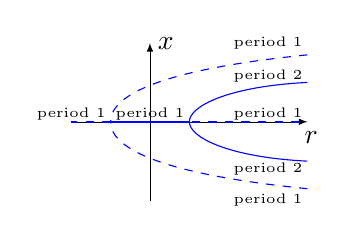
\begin{tikzpicture}
\draw [ultra thin,latex-](0,1.5) -- (0,-0.5);
\draw [ultra thin,-latex](-1,0.5) -- (2,0.5);
\draw [color=blue, thick](-0.5,0.5) -- (0.5,0.5);
\draw [color=blue, dashed, thick](-0.5,0.5) -- (-1.,0.5);
\draw [color=blue, dashed, thick](1.9,0.5) -- (0.5,0.5);
\draw [color=blue](2,0) .. controls (1,0.05) and (0.5,0.3) .. (0.5,0.5);
\draw [color=blue](2,1) .. controls (1,0.95) and (0.5,0.7) .. (0.5,0.5) node (v1) {};
\draw [color=blue, dashed](2,-0.35) .. controls (0,-0.15) and (-0.5,0.2) .. (-0.5,0.5);
\draw [color=blue, dashed](2,1.35) .. controls (0,1.15) and (-0.5,0.8) .. (-0.5,0.5) node (v1) {};
\node at (2.05,0.3) {$r$};
\node at (0.2,1.5) {$x$};
\node at (0,0.6) {{\tiny period 1}};
\node at (-1,0.6) {{\tiny period 1}};
\node at (1.5,-0.5) {{\tiny period 1}};
\node at (1.5,1.5) {{\tiny period 1}};
\node at (1.5,0.6) {{\tiny period 1}};
\node at (1.5,1.075) {{\tiny period 2}};
\node at (1.5,-0.1) {{\tiny period 2}};
\end{tikzpicture}
\end{center}

\subsection{(Supercritical) Neimark-Sacker bifurcation}
\emph{A bifurcation when the FP changes stability via a pair of complex eigenvalues}
Discrete-time counterpart to the Hopf bifurcation.\\
$z(t_{n+1}) = (1+\beta)e^{i\Theta(\beta)}z(t_n)+c(\beta)z(t_n)|z(t_n)|^2 + \mathcal{O}(|z(t_n)|^4)$. For $\beta<0$ the origin is a asymptotically stable FP (weakly stable at $\beta=0$) and unstable for $\beta>0$. Unique stable LC for $\beta>$ with radius $\sqrt{b}$.
